\documentclass[9pt,ignorenonframetext,xcolor=dvipsnames]{beamer}
\setbeamertemplate{caption}[numbered]
\setbeamertemplate{caption label separator}{: }
\setbeamercolor{caption name}{fg=normal text.fg}
\beamertemplatenavigationsymbolsempty
\usepackage{lmodern}
\usepackage{amssymb,amsmath}
\usepackage{ifxetex,ifluatex}
\usepackage{fixltx2e} % provides \textsubscript
\ifnum 0\ifxetex 1\fi\ifluatex 1\fi=0 % if pdftex
  \usepackage[T1]{fontenc}
  \usepackage[utf8]{inputenc}
\else % if luatex or xelatex
  \ifxetex
    \usepackage{mathspec}
  \else
    \usepackage{fontspec}
  \fi
  \defaultfontfeatures{Ligatures=TeX,Scale=MatchLowercase}
\fi
\usetheme[]{metropolis}
\usefonttheme{serif}
% use upquote if available, for straight quotes in verbatim environments
\IfFileExists{upquote.sty}{\usepackage{upquote}}{}
% use microtype if available
\IfFileExists{microtype.sty}{%
\usepackage{microtype}
\UseMicrotypeSet[protrusion]{basicmath} % disable protrusion for tt fonts
}{}
\newif\ifbibliography
\hypersetup{
            pdftitle={임상연구 설계와 분석을 위한 통계 방법},
            pdfauthor={, Ph.D., Senior researcher},
            colorlinks=true,
            linkcolor=Maroon,
            citecolor=Blue,
            urlcolor=blue,
            breaklinks=true}
\urlstyle{same}  % don't use monospace font for urls

% Prevent slide breaks in the middle of a paragraph:
\widowpenalties 1 10000
\raggedbottom

\AtBeginPart{
  \let\insertpartnumber\relax
  \let\partname\relax
  \frame{\partpage}
}
\AtBeginSection{
  \ifbibliography
  \else
    \let\insertsectionnumber\relax
    \let\sectionname\relax
    \frame{\sectionpage}
  \fi
}
\AtBeginSubsection{
  \let\insertsubsectionnumber\relax
  \let\subsectionname\relax
  \frame{\subsectionpage}
}

\setlength{\parindent}{0pt}
\setlength{\parskip}{6pt plus 2pt minus 1pt}
\setlength{\emergencystretch}{3em}  % prevent overfull lines
\providecommand{\tightlist}{%
  \setlength{\itemsep}{0pt}\setlength{\parskip}{0pt}}
\setcounter{secnumdepth}{0}
\usepackage{kotex}
\usepackage{placeins}
\usepackage{enumerate}
\usepackage{amssymb}
\usepackage{amsmath}
\usepackage{mathtools}
\usepackage{float}
% \usepackage{setspace}\doublespacing
\usepackage{relsize}
\usepackage{bigints}
\usepackage{bm}
\usepackage{booktabs}
\usepackage{dcolumn}
\usepackage{array}
\usepackage[font=scriptsize,labelfont=bf]{caption}
\usepackage{gensymb}
\usepackage{makecell}
\usepackage{graphicx}
\usepackage{rotating}
\usepackage{pgf}
\usepackage{pgfpages}
\usepackage{textpos}

\renewcommand\theadalign{cb}
\renewcommand\theadfont{\bfseries}
\renewcommand\theadgape{\Gape[4pt]}
\renewcommand\cellgape{\Gape[4pt]}
\DeclareMathAlphabet{\mathpzc}{OT1}{pzc}{m}{it}

\renewcommand\theadalign{cb}
\renewcommand\theadfont{\bfseries}
\renewcommand\theadgape{\Gape[4pt]}
\renewcommand\cellgape{\Gape[4pt]}

\newcolumntype{L}[1]{>{\raggedright\let\newline\\
\arraybackslash\hspace{0pt}}m{#1}}
\newcolumntype{C}[1]{>{\centering\let\newline\\
\arraybackslash\hspace{0pt}}m{#1}}
\newcolumntype{R}[1]{>{\raggedleft\let\newline\\
\arraybackslash\hspace{0pt}}m{#1}}
\newcolumntype{P}[1]{>{\raggedright\tabularxbackslash}p{#1}}
\newcommand{\specialcell}[2][c]{%
  \begin{tabular}[#1]{@{}c@{}}#2\end{tabular}}

\newlength{\wideitemsep}
\setlength{\wideitemsep}{\itemsep}
\addtolength{\wideitemsep}{0.1cm}
\let\olditem\item
\renewcommand{\item}{\setlength{\itemsep}{\wideitemsep}\olditem}

% \setbeameroption{show notes on second screen=bottom}
\setbeameroption{show notes}
\setbeamertemplate{note page}[plain]
\setbeamertemplate{navigation symbols}{}
\setbeamertemplate{headline}[default]


% \setbeamertemplate{headline}{%
% \leavevmode%
  % \hbox{%
    % \begin{beamercolorbox}[wd=\paperwidth,ht=3ex,dp=1.125ex, right]{palette quaternary}%
    % \usebeamercolor[fg]{navigation symbols}\insertslidenavigationsymbol%
		% \insertframenavigationsymbol%
		% \insertsubsectionnavigationsymbol%
		% \insertsectionnavigationsymbol%
		% \insertdocnavigationsymbol%
		% \insertbackfindforwardnavigationsymbol%
    % \end{beamercolorbox}%
  % }
% }

\addtobeamertemplate{frametitle}{}{
\leavevmode%
  \hbox{%
    \begin{beamercolorbox}[wd=\paperwidth,ht=3ex,dp=1.125ex, right]{palette quaternary}%
    \usebeamercolor[fg]{navigation symbols}\insertslidenavigationsymbol%
		\insertframenavigationsymbol%
		\insertsubsectionnavigationsymbol%
		\insertsectionnavigationsymbol%
		\insertdocnavigationsymbol%
		\insertbackfindforwardnavigationsymbol%
    \end{beamercolorbox}%
  }
}

\setbeamertemplate{footline}
{
  \leavevmode%
  % \includegraphics[width = \paperwidth, height = 0.5cm]{KIOM-BAR.png}
  % \vskip-10pt
  \hbox{%
  \begin{beamercolorbox}[wd=0.3\paperwidth,ht=3ex,dp=1ex,center]{author in head/foot}%
    \usebeamerfont{author in head/foot}{Boncho Ku}
  \end{beamercolorbox}%
  \begin{beamercolorbox}[wd=0.3\paperwidth,ht=3ex,dp=1ex,center]{title in head/foot}%
    \usebeamerfont{title in head/foot}{임상연구 설계와 분석을 위한 통계 방법}
  \end{beamercolorbox}%
  \begin{beamercolorbox}[wd=.4\paperwidth,ht=3ex,dp=1ex,center]{date in head/foot}%
    secondmoon@kiom.re.kr\hspace{0.5cm}\insertframenumber{} / \inserttotalframenumber\hspace*{1ex}
  \end{beamercolorbox}}%
  \vskip0pt%
}

\title{임상연구 설계와 분석을 위한 통계 방법}
\author{\textbf{Boncho Ku}, Ph.D., Senior researcher}
\institute{KM Fundamental Research Division, Korea Institute of Oriental Medicine}
\date{\(16^{\mathrm{th}}\) November, 2017}

\begin{document}
\frame{\titlepage}

\section{\texorpdfstring{Chapter I:
\LARGE{Overview of Statistics and Study Design}}{Chapter I: }}\label{chapter-i}

\begin{frame}{What is Statistics?}

\LARGE{\textbf{Most researchers or people think}}

\large{Statistics makes us insane...}

\LARGE{\textbf{However}}

\large{Statistics sometimes gives us very useful information from data!!}

\large{So then, what is statistics??} \vspace{0.5cm}

\begin{columns}
  \begin{column}{0.4\textwidth}
    \begin{center}
      
\includegraphics[width = 2.5cm, height = 2.5cm]{StatisticsWords_Meg.jpg}
    \end{center}
  \end{column}
  \begin{column}{0.6\textwidth}
    \begin{center}
      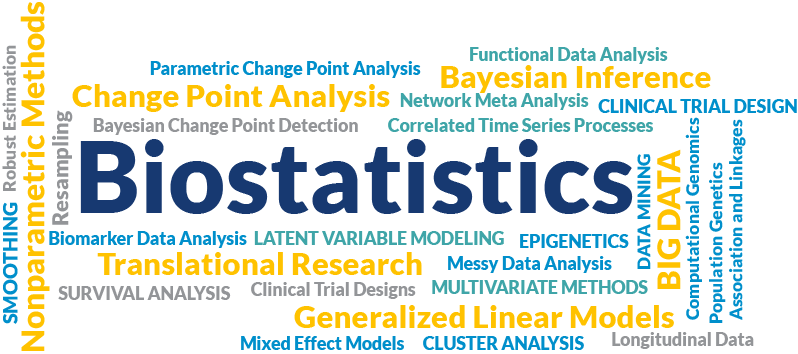
\includegraphics[width = 4.8cm, height = 2.5cm]{wordcloud-biostatics.png}
    \end{center}
  \end{column}
\end{columns}

\tiny{$^{\dagger}$ Each wordcloud was cited from \href{http://blog.trident.edu/-temporary-slug-8756cc7e-1d1b-458e-94e2-3ff603f80c9e}{Trident University International} and \href{http://www.augusta.edu/mcg/dphs/biostats/research/index.php}{Augusta University}, respectively.}

\end{frame}

\begin{frame}{Main Pillars of Statistics}

\LARGE

\begin{enumerate}
\def\labelenumi{\arabic{enumi}.}
\tightlist
\item
  Data

  \begin{itemize}
  \tightlist
  \item
    Investigation, experiment, and survey
  \item
    Gathering numbers (for quantitative analysis)
  \end{itemize}
\item
  Description or Summarization

  \begin{itemize}
  \tightlist
  \item
    Table, chart, and so on
  \item
    Based on summarized statistics (e.g.~mean, standard deviation,
    median, \ldots{})
  \end{itemize}
\item
  Inference

  \begin{itemize}
  \tightlist
  \item
    Numerous statistical tests and models based on probability theory
  \item
    e.g.~two-sample t-test, ANOVA, ANCOVA, regression, and so on
  \end{itemize}
\end{enumerate}

\end{frame}

\section{Type of Studies}\label{type-of-studies}

\begin{frame}{Overview}

\LARGE{Study or trial?}

\end{frame}

\begin{frame}{Overview}

\begin{block}{Study}

자료의 수집과 분석 목적이 학술적 목적에 국한된 모든 종류의 연구 및 실험

\end{block}

\begin{block}{Trial}

자료의 수집과 분석 목적이 이윤추구 또는 허가에 목적이 있는 임상시험

\end{block}

\end{frame}

\begin{frame}{Observational Study}

\begin{block}{Cross-sectional study (단면적 관찰연구)}

\begin{enumerate}
\def\labelenumi{\arabic{enumi}.}
\tightlist
\item
  prevalence study
\item
  Diagostic test
\item
  Ecological study
\item
  Validity, Reliability, and agreement study
\end{enumerate}

\end{block}

\begin{block}{Longitudinal study (종단적 관찰연구)}

\begin{enumerate}
\def\labelenumi{\arabic{enumi}.}
\tightlist
\item
  Prospective study
\item
  Retrospective study
\end{enumerate}

\end{block}

\end{frame}

\begin{frame}{Experimental Study}

\begin{block}{Randomized controlled trial}

\end{block}

\begin{block}{Pilot study}

\end{block}

\begin{block}{Exploratory study}

\end{block}

\begin{block}{Confirmative study}

\end{block}

\end{frame}

\section{Type of outcome variables}\label{type-of-outcome-variables}

\begin{frame}{Primary outcomes}

\end{frame}

\begin{frame}{Secondary outcomes}

\end{frame}

\begin{frame}{Surrogate variables}

\end{frame}

\begin{frame}{Global assessment variable}

\end{frame}

\section{Sample size calculation}\label{sample-size-calculation}

\begin{frame}{Overview}

\begin{block}{Two approaches}

\begin{enumerate}
\def\labelenumi{\arabic{enumi}.}
\tightlist
\item
  Based on the marginal error rate \(\rightarrow\) population based
  observational study
\item
  Based on the effectiveness between concerning groups \(\rightarrow\)
  experimental study
\end{enumerate}

\textbf{Both approaches are based on previous studies}

\textbf{Is your study entirely new?}

\end{block}

\end{frame}

\begin{frame}{Observational study}

\end{frame}

\begin{frame}{Observational study: prevalence study}

\end{frame}

\begin{frame}{Observational study: prevalence study}

\end{frame}

\begin{frame}{Parallel design}

\end{frame}

\begin{frame}{\(2\times 2\) cross-over design}

\end{frame}

\begin{frame}{Factorial design}

\end{frame}

\section{Multiple comparison}\label{multiple-comparison}

\begin{frame}{What makes data significant?}

\begin{enumerate}
\def\labelenumi{\arabic{enumi}.}
\tightlist
\item
  Data themselves contain unexpected errors
\item
  Bias
\item
  Just conincidence
\item
  Our hypothesis is working
\end{enumerate}

\end{frame}

\begin{frame}{Torturing data}

\end{frame}

\section{Statistical Analysis}\label{statistical-analysis}

\begin{frame}{Overview}

\end{frame}

\begin{frame}{Independent two sample t-test}

\begin{enumerate}
\def\labelenumi{\arabic{enumi}.}
\tightlist
\item
  Too easy, but very useful methodology for the comparison of sample
  means between two groups
\end{enumerate}

\end{frame}

\begin{frame}{Analysis of Variance (ANOVA)}

\end{frame}

\begin{frame}{Analysis of Covariance (ANCOVA)}

\end{frame}

\begin{frame}{Simple or multiple regression}

\end{frame}

\begin{frame}{Repeated Measures ANOVA}

\end{frame}

\begin{frame}{Linear mixed effects model}

\end{frame}

\begin{frame}{Reliability analysis}

\begin{block}{Cohen's \(\kappa\)}

\end{block}

\begin{block}{Cronbach's \(\alpha\)}

\end{block}

\begin{block}{Intra Class Correlation (ICC)}

\end{block}

\end{frame}

\end{document}
